\documentclass[11pt,a4paper,oneside,titlepage,openright]{book}
\usepackage{float}
\usepackage{graphicx}
\usepackage{titlesec}
\usepackage[english]{babel}
\usepackage[T1]{fontenc}
\usepackage{fancyhdr}
\usepackage{subfigure}
\pagestyle{empty}
\usepackage[utf8]{inputenc}
\usepackage{titling}
\usepackage{listings}
\usepackage{amsmath}
\usepackage{amsfonts}
\usepackage{xcolor}

\definecolor{mGreen}{rgb}{0,0.6,0}
\definecolor{mGray}{rgb}{0.5,0.5,0.5}
\definecolor{mPurple}{rgb}{0.58,0,0.82}
\definecolor{backgroundColour}{rgb}{0.95,0.95,0.92}

\lstdefinestyle{CStyle}{
    backgroundcolor=\color{backgroundColour},   
    commentstyle=\color{mGreen},
    keywordstyle=\color{magenta},
    numberstyle=\tiny\color{mGray},
    stringstyle=\color{mPurple},
    basicstyle=\footnotesize,
    breakatwhitespace=false,         
    breaklines=true,                 
    captionpos=b,                    
    keepspaces=true,                 
    numbers=left,                    
    numbersep=5pt,                  
    showspaces=false,                
    showstringspaces=false,
    showtabs=false,                  
    tabsize=2,
    language=C
}



%%ENVIRONMENT FOR ABSTRACT
\newenvironment{abstract}
{\cleardoublepage\null \begin{center}
\bfseries \abstractname \end{center}}
	{\vfill\null}
	
%%DEFINITION FOR FIRST PAGE
\makeatletter

\renewcommand{\maketitle}{%
  \let\footnotesize\small
  \let\footnoterule\relax
  \let\footnote\thanks
  \chapter*{\vspace{-3cm}\makebox[\linewidth]{\@title}}
  \begin{center}
    
\includegraphics[width=5cm]{logo}
    \vskip\dimexpr 7em-40\p@\relax%
    {\large \lineskip 0.4em%
     \textsc{Bachelor of Science in Mathematical Engineering}\\
     \vskip 0.4cm
     \Large\textsc{Bachelor degree thesis}	\\
     \vskip 1cm
     \Huge\textbf{Analysis of matrix vector product}
     \begin{tabular}[t]{c}  \@author \end{tabular}\par}%
     \vskip 3cm
    \noindent
    \parbox[t]{.5\textwidth}{\raggedright
    \large{Supervisors:}\\
    \large{Prof. Stefano Berrone\\ Dr. Federico Tesser}}
    \hfill
    \parbox[t]{.3\textwidth}{\raggedleft
    \large Candidate:\\
    \large{Ludovico Bessi}
    }%
    \vskip 10.7em%
    {\large \@date \par}%
  \end{center}\par
  \@thanks
  \vfill\null\setcounter{footnote}{0}
  \thispagestyle{empty}\addtocounter{page}{-1}
}
\makeatother

\begin{document} 
\title{POLITECNICO DI TORINO}
\author{}
\date{July 2019}
\maketitle

%%DEDICA
\begin{flushright}
\null\vspace{\stretch{1}}
\textit{Ai miei genitori}
\vspace{\stretch{2}}\null
\end{flushright}


%%ABSTRACT
\begin{abstract}
Comparison between different self-made implementations of the dense matrix vector product and Eigen's library implementation, using different optimizations flags on a single core.\\ After getting to the theoretical limit of performance on our machine, I addressed scalability by running the code in parallel using OpenMP. 
\end{abstract}

\tableofcontents


%%CAPITOLO 1
\chapter{Introduction}
In this first chapter I will introduce the main ideas to understand three different implementations of the code, plus the tools used to analyze them. \\
Let $A$ be a $n\times n$ dense matrix and v be a vector of $n$ entries. We define the \textbf{kernel} as the following operation: 
$$ result[i] = result[i] + A[i,j]*vector[i]$$ 
The kernel is indeed very simple, so there is not much mathematical machinery that can be employed to speed up the calculation. \\
However, I will show how to write it in slightly different ways to exploit the cache and pipe dimension.  \\
When using the g++ compiler, we can set different optimization flags such as: O0, O1, O2 and O3. \\
O$0$ is the default one, and no optimization is done. From here, the higher the number the better the compiler optimizes the code.\\
The code comparison will then be done with different optimization flags and different size of matrices. The reason for the latter is that there exists a number $n \in \mathbb{N}$ such that all our data will be saved in the Cache, thus speeding up the algorithm. 


\section{STREAM} 
STREAM is a simple synthetic benchmark program that measures sustainable memory bandwidth in MB/s and the corresponding computation rate for  vector kernels. \\
 Having an estimate of bandwidth is very important because it lets us calculate the performance of our code relatively to the hardware. 
By running a python script, I calculated that our bandwidth on average is: 6000 MB/s.


\section{LIKWID}
LIKWID is a set of command line tools supporting software developers, benchmarkers and application users to get the best performance on a given system.
One of the main tool is \textbf{likwid-perfctr}, that offers access to hardware performance counters and derives metrics from the raw counts. 
By running likwid-perfctr, we can profile our code. The following screenshot is an example of an output: 

\begin{center}
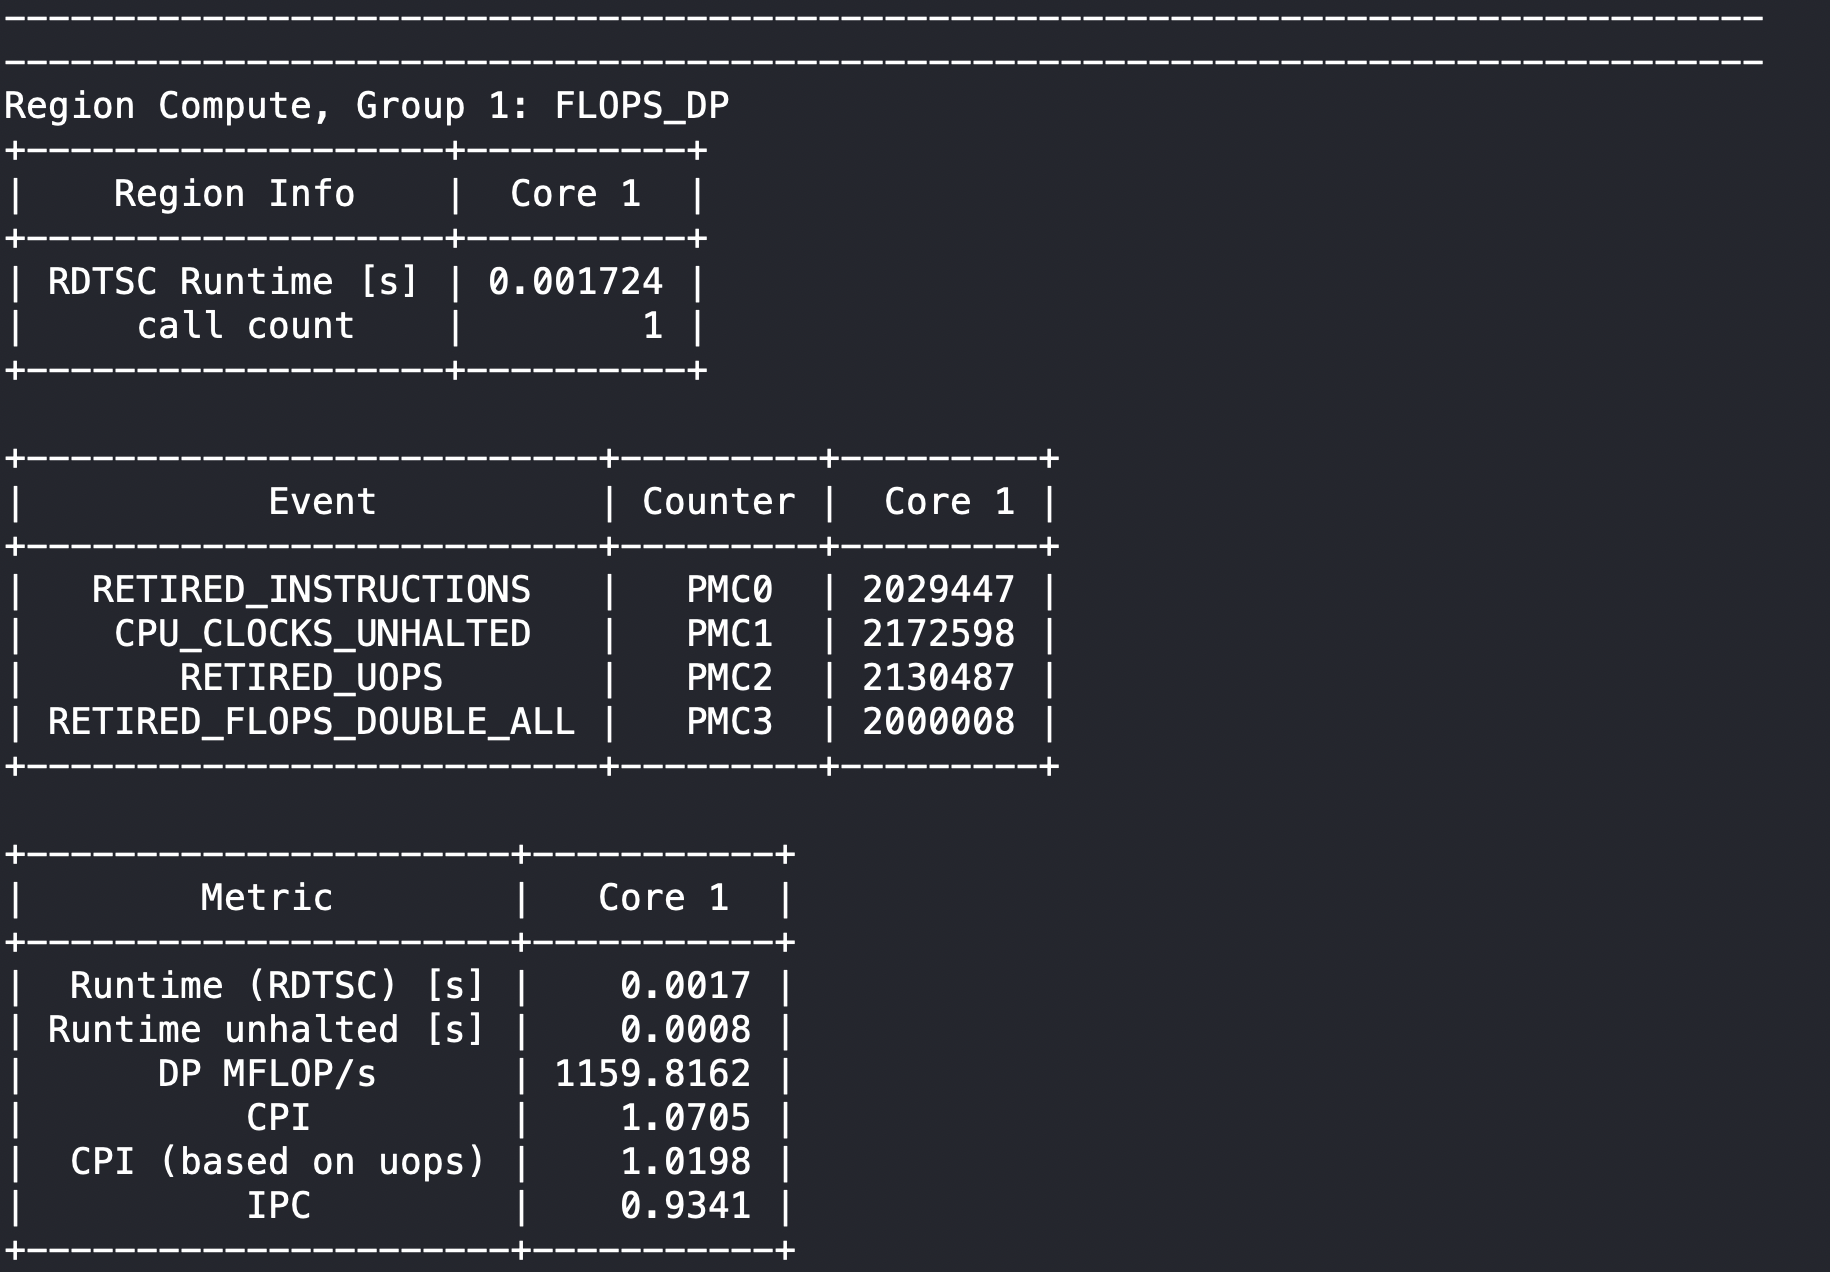
\includegraphics[width=10cm, height=8cm]{scree_lik_perf}
\end{center}

A brief explanation of all the metrics: 

\begin{itemize}
\item{\textbf{RETIRED\_INSTRUCTIONS}: instructions completely executed between two clocktick event samples.}
\item{\textbf{CPU\_CLOCKS\_UNHALTED}: number of cycles where CPU was not halted.}
\item{\textbf{RETIRED\_UOPS}: number of low-level hardware operations.}
\item{\textbf{RETIRED\_FLOPS\_DOUBLE\_ALL}: number of completely executed floating point operation per second  }
\item{\textbf{Runtime (RDTSC) [s]}: counts the number of cycles since reset. }
\item{\textbf{Runtime unhalted [s]}: counts the number of cycles since reset when CPU was not halted.}
\item{\textbf{DP MFLOP/s}:  number of double precision MFLOP/s.}
\item{\textbf{ CPI}: number f cycles per instruction retired.}
\item{\textbf{CPI (based on uops)}: Calculation of CPI based on uops.}
\item{\textbf{ IPC }: number of instructions per cycles}
\end{itemize}

Below some useful formulas that provide more insights into how these numbers are related to each other: 
\begin{itemize}
\item DP MFLOP/s = 1.0E-06*(RETIRED\_FLOPS\_DOUBLE\_ALL)/time
\item CPI = CPU\_CLOCKS\_UNHALTED/RETIRED\_INSTRUCTIONS
\item CPI (based on uops) = CPU\_CLOCKS\_UNHALTED/RETIRED\_UOPS
\item IPC = RETIRED\_INSTRUCTIONS/CPU\_CLOCKS\_UNHALTED
\end{itemize}

To understand and use the performance properties of the hardware, it is important to know the machine's topology: \textbf{likwid-topology} gives us information about: 
\begin{itemize}
\item \textbf{Thread topology}: how threads are concurrently executed and split in subprocesses. 
\item \textbf{Cache topology}: how processors share the cache hierarchy.
\item \textbf{Cache properties}: detailed information about all cache levels.
\end{itemize}

Below an example of the output with information about HW and thread topology:\\
\begin{center}
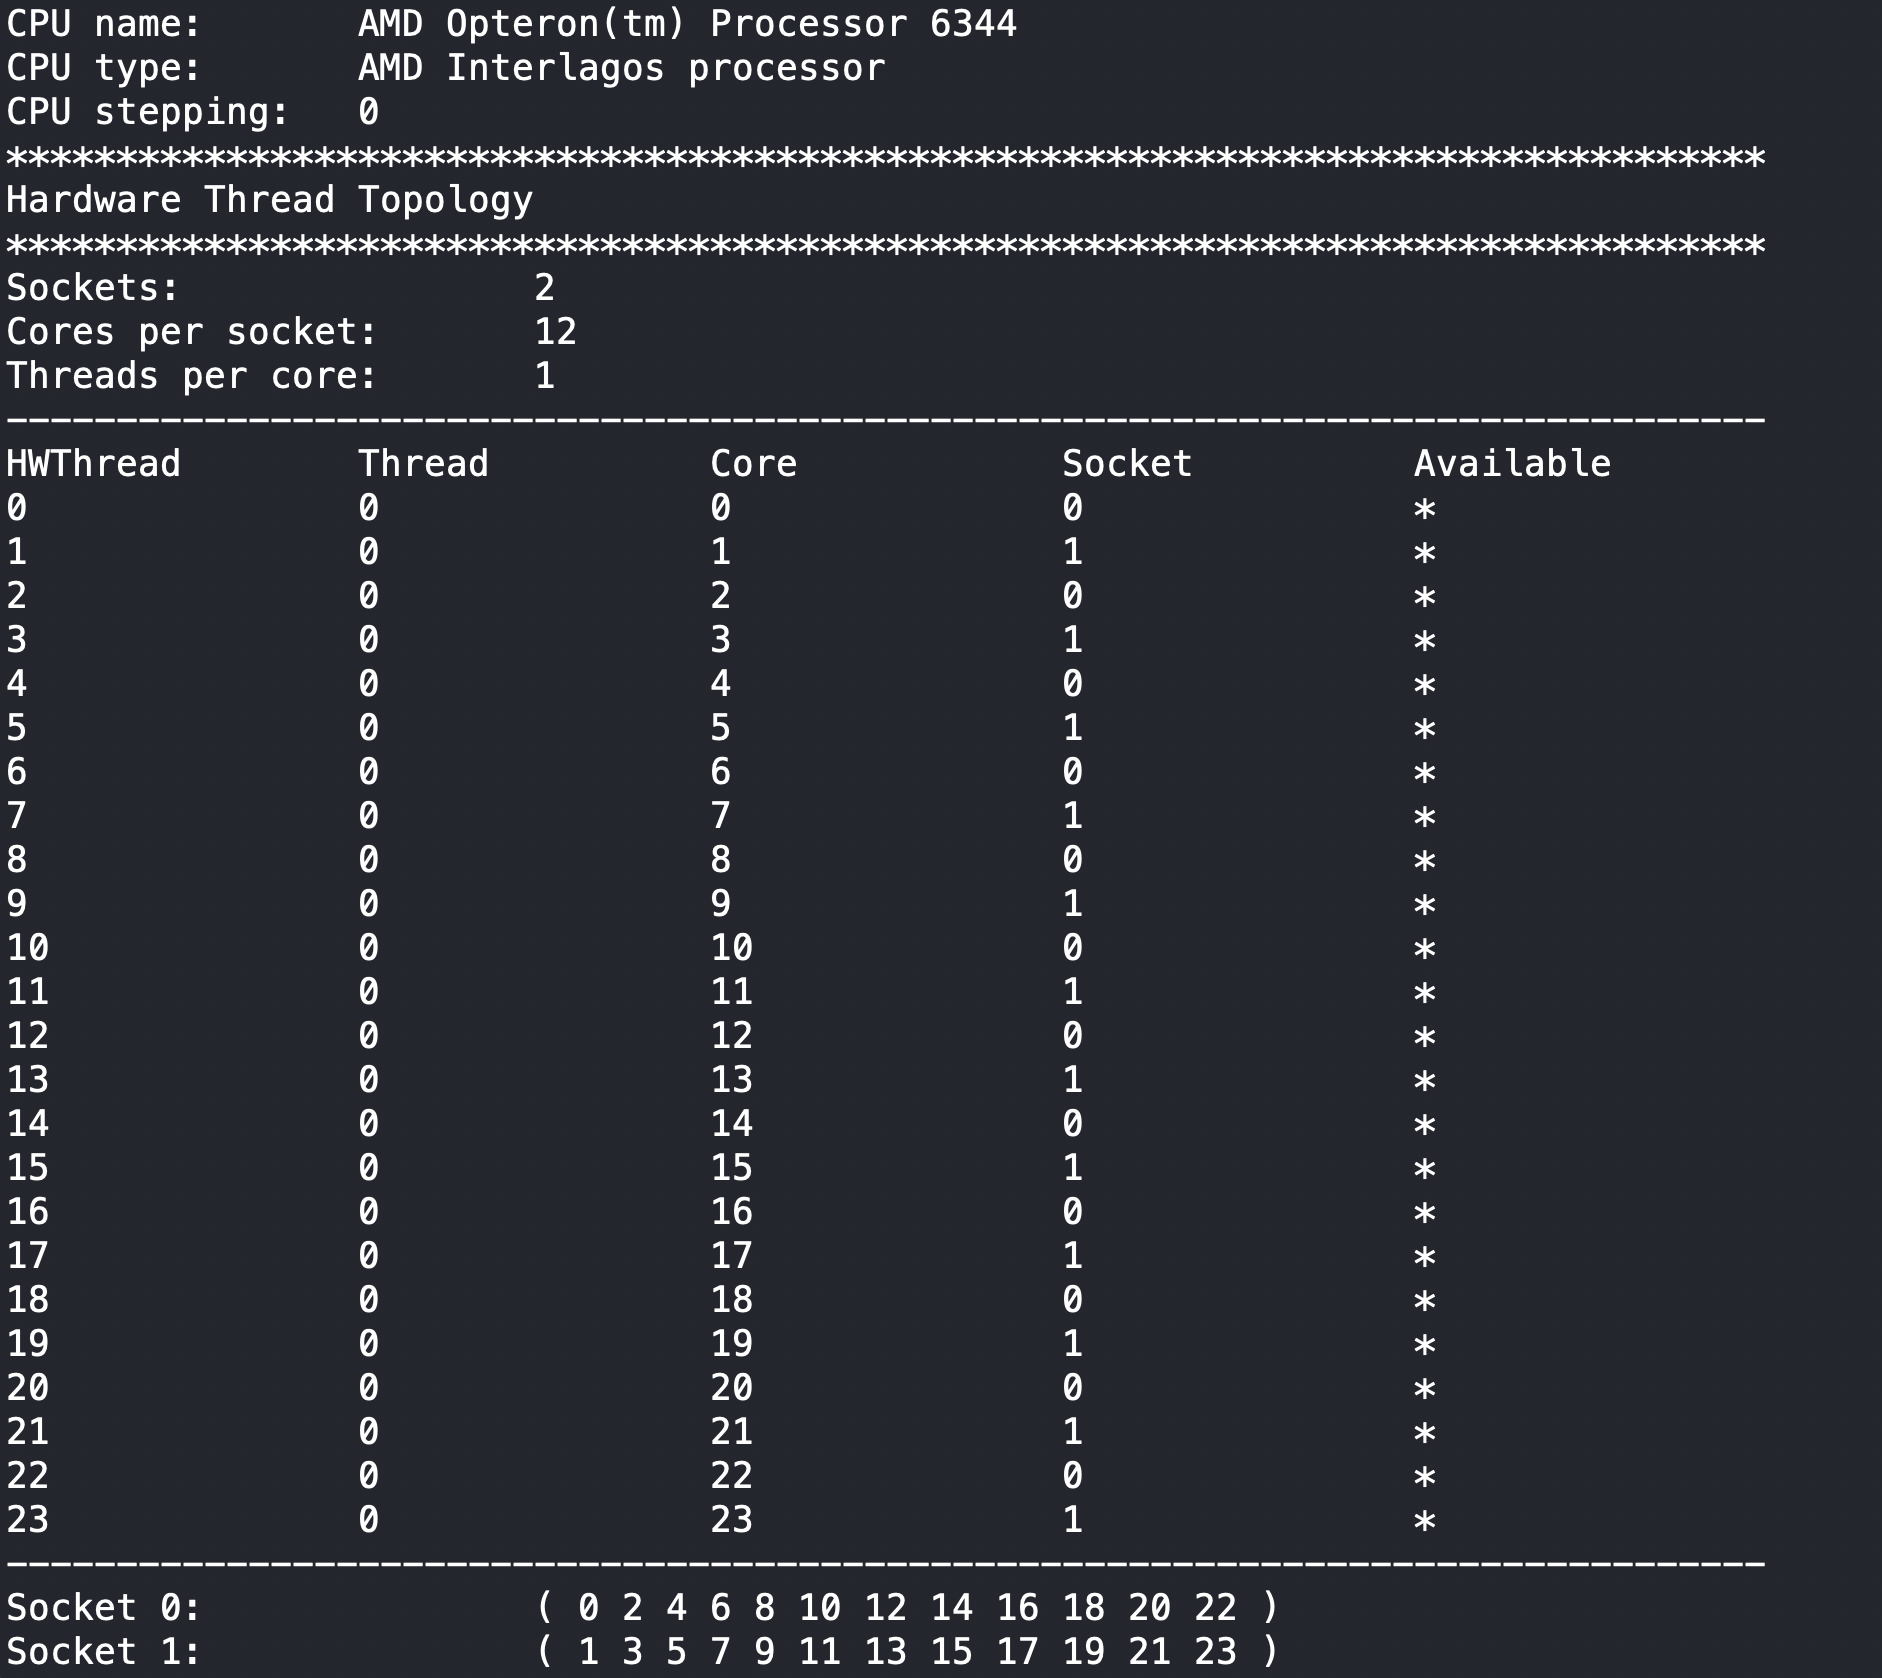
\includegraphics[width=10cm, height=8cm]{topology_1}
\end{center}
Another picture with information on cache levels:\\
\begin{center}
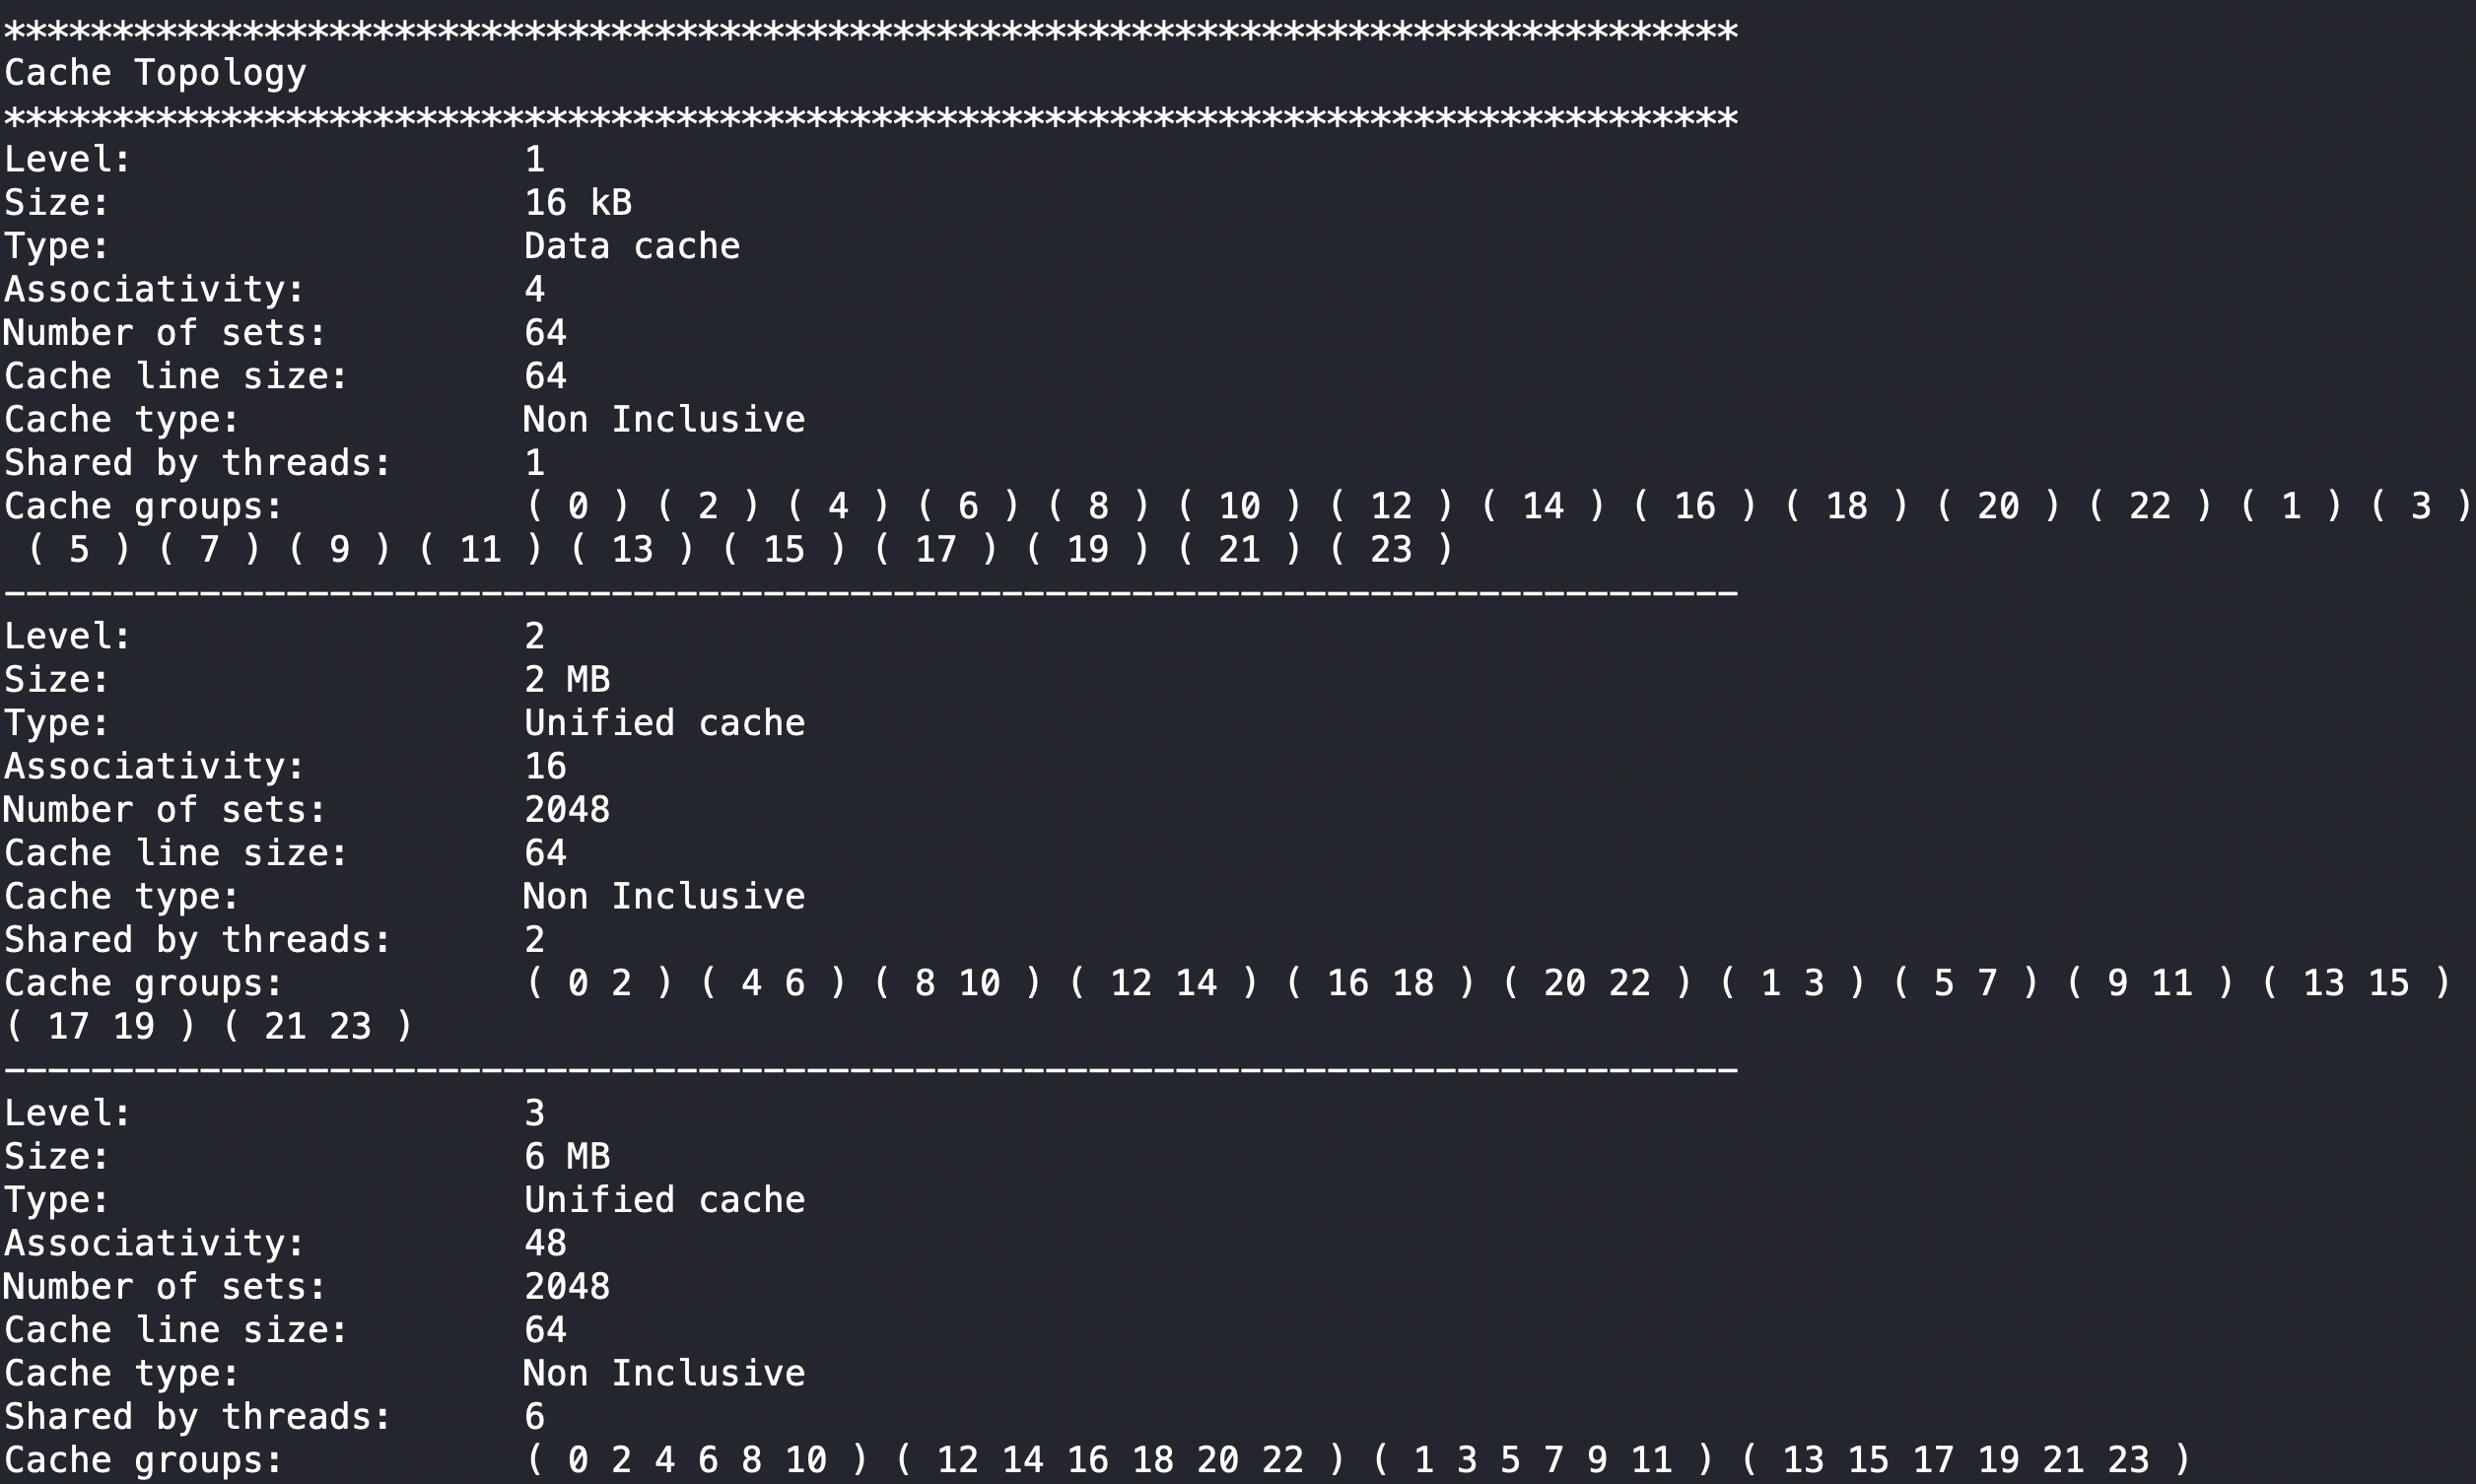
\includegraphics[width=10cm, height=8cm]{topology_2}
\end{center}

Lastly, likwid let us change the maximum and minimum frequency of our CPU. To have the least amount of oscillations when running our code, we set both at 2.6GHz, which is the maximum frequency allowed by our machine.

\section{Eigen}
Our main goal is to see how our code measures against Eigen's. 
Eigen is a library written in C++ which provides algorithms for fast matrix algebra, such as: dense and sparse product of matrix and vectors, matrix decomposition, space transformations. \\This library is widely used by many projects and is the result of the work of experts starting at least from 2009. Given this premises, it seems very difficult to get close to their performance. However, even matching it will be a great accomplishment and would show that there is still work to be done to improve it. 

\section{Roof-line model}
The Roofline model is a performance model used to provide estimates of a given computer kernel. 
It can be visualized by plotting floating point performance as a function of arithmetic intensity. 
Below an example of such a plot taken by \cite{roofmodel}.

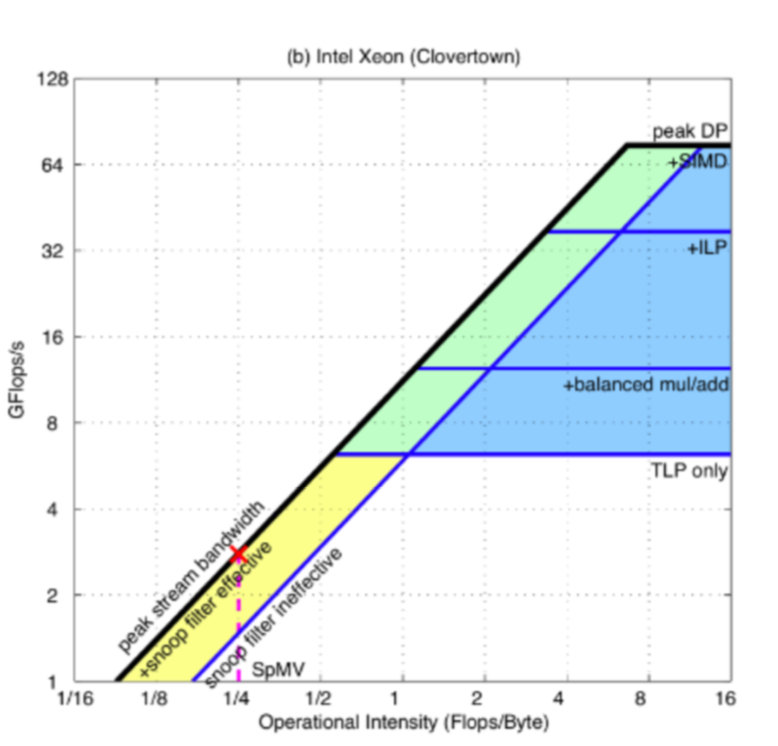
\includegraphics[width=10cm, height=8cm]{roof_example}
\\This model is used to determine the two main bottlenecks: bandwidth and core. It works under the assumption that data is already saved in cache and there  is no latency. It depends on empirical measurements, so it is inherently subject to error. 
It plots the performance of the code as dependent variable of computational intensity, below I will explain how to calculate such values using the tool described at the beginning of the chapter. 
\\
The peak performance can be calculated using the following formula, where $n$ is the number of cores, $F$ is the number of floating point instructions for cycle, $v$ is the clock speed and $S$ is the SIMDY feature, for now we are not concerned about this last term. 
$$ P_{peak} = n * F * S * v $$ 

We can also define the maximum performance reached by our machine with the following formula, where $f_{max}$ is the maximum frequency of the CPU of our machine, $\frac{n_{operations}}{n_{cycles}}$ is the number of operations per cycle. 
$$P_{max} = f_{max} * \frac{n_{operations}}{n_{cycles}}$$ 

In our case, the result is then just 2.6$\frac{Gflops}{s}$.
However, this is just the theoretical limit: our performance P actually is: 

$$ P = min(P_{max}, \text{Bandwidth * computational intensity}) $$

In this formula, computational intensity is s a measure of floating-point operations (FLOPs) performed by a given code (or code section) relative to the amount of memory accesses (Bytes) that are required to support those operations. \\
We shall see how it is indeed the deciding factor when evaluating different algorithms, because in this framework we ideally want to build an an algorithm such as that the value $\textbf{Bandwidth * computational intensity}$ reaches $P_{max}$.\\

With this idea in mind, I developed three different implementations of the dense matrix vector product:

\begin{itemize}
\item \textbf{Naive implementation}: the classic implementation without much thought, still useful to benchmark against to check progress. 
\item \textbf{Temporary variable}: using a temporary variable to always keep in cache a value to lessen the number of fetches from memory. 
\item \textbf{Loop unrolling}: splitting up the loop manually to exploit pipe levels, that means keeping the pipe occupied avoiding  downtime. 
\end{itemize}

With the last implementation, we managed to get to the theoretical limit. After that, we adressed scalability. That is, we looked at how our kernel worked in parallel using OpenMP.




%%CAPITOLO 2
\chapter{Naive implementation}

The naive implementation is just that, the simplest code one can develop to solve this problem, below the .C file:
\lstinputlisting[style=CStyle]{naive_without_tmp.c}
The computational intensity in this case is $\frac{2}{32}\frac{Flops}{Bytes}$. 
\\Before blindly applying the formulas seen in chapter one, there are some key insights to understand. until we get to the final implementation, we are not exploiting pipelines of sum and product. In short, this means that we are not allowing the processor to execute these basic operations in parallel. It follows that $P_{max}$ is limited by a factor of $8$, because the size of the pipe for sum and of product are 4 each.
We then have that $P_{max}= \frac{2.6}{8} \frac{Gflops}{s} $, and this is a major bottleneck of our program, because $\textbf{Bandwitdht} * \textbf{computational intensity} = 6*\frac{1}{16} = 0.375 \frac{Gflops}{s} $. We will tackle the bottleneck in chapter 4.

Using likwid-topology, we find the following sizes for the cache: 
\begin{itemize}
\item L1: 16 kB
\item L2: 2 MB
\item L3: 6 MB
\end{itemize}
We are going to focus our attention on the L1 and L2 cache levels, which are the fastest. In short: if the elements we are working with are saved there, we can access them faster than usual.  For dense matrices, L2 is actually faster than L1. I am going to repeat the same analysis with two different matrices $A_1$ and $A_2$ of size respectively $n_1 = 40$ and  $n_2 = 400$.  The first matrix can be saved in L1, the second one in L2 and the one with $n=1000$ is saved in memory.  

 
\section{Different optimization flags comparison}
I will now analyze the code compiling it with different flags: O0, O1, O2 and O3 and $n = 1000$.

I am going to focus on the DP Mflops/s, the higher the number the faster the result. 
\begin{itemize}
\item[\textbf{O0}] 328  Mflops/s
\item[\textbf{O1}] 740 Mflops/s
\item[\textbf{O2}] 720 Mflops/s
\item[\textbf{O3}] 761 Mflops/s
\end{itemize}


\section{Decreasing matrix dimension} 
By changing the matrix dimension, we get different and interesting results. 

\subsection{ n = 44}

\begin{itemize}
\item[\textbf{O0}] 213  Mflops/s
\item[\textbf{O1}] 370 Mflops/s
\item[\textbf{O2}] 345 Mflops/s
\item[\textbf{O3}] 368 Mflops/s
\end{itemize}


\subsection{ n = 400}

\begin{itemize}
\item[\textbf{O0}] 328  Mflops/s
\item[\textbf{O1}] 948 Mflops/s
\item[\textbf{O2}] 941 Mflops/s
\item[\textbf{O3}] 936 Mflops/s
\end{itemize}




%%CAPITOLO 3
\chapter{Temporary variable}

We can improve the code described in chapter two, introducing a temporary variable in the following way: 
\lstinputlisting[style=CStyle]{naive_with_tmp.c}

At first glance, It may seem we are just wasting precious cache space with another double variable but it turns out this change doubles the computational intensity with respect to the first algorithm. \\
The key take away is that our kernel does not change even with the addition of the $\textit{tmp}$ variable: this time we can skip the fetching and loading of this variable, because when entering the second for loop it is already in the cache. This means that the computational intensity becomes $\frac{1}{8}\frac{Flops}{Bytes}$. 
However, we still have not solved the pipeline's problem described in the previous chapter. \\
This means that even though we doubled the computational intensity our bottleneck is still $P_{max}$ due to the coefficient $\frac{1}{8}$.  
Nevertheless, by compiling the code we still manage to improve, as seen in the next section. 

\section{Different optimization flags comparison}
I will now analyze the code compiling it with different flags: O0, O1, O2 and O3 and $n = 1000$.

\begin{itemize}
\item[\textbf{O0}] 328  Mflops/s
\item[\textbf{O1}] 344 Mflops/s
\item[\textbf{O2}] 704 Mflops/s
\item[\textbf{O3}] 766 Mflops/s
\end{itemize}

\section{Decreasing matrix dimension} 

\subsection{ n = 44}
\begin{itemize}
\item[\textbf{O0}] 229  Mflops/s
\item[\textbf{O1}] 276 Mflops/s
\item[\textbf{O2}] 357 Mflops/s
\item[\textbf{O3}] 348 Mflops/s
\end{itemize}

\subsection{ n = 400}

\begin{itemize}
\item[\textbf{O0}] 332  Mflops/s
\item[\textbf{O1}] 345 Mflops/s
\item[\textbf{O2}] 937 Mflops/s
\item[\textbf{O3}] 961 Mflops/s
\end{itemize}



%CAPITOLO 4 
\chapter{Loop unrolling}
With this code, I finally manage to exploit the sum and product pipelines, thus reaching $P_{max}$ = 2.6 GHz, then the bottleneck must be in the other term, which depends on the computational intensity of the algorithm. 
The code can be found below: 
\lstinputlisting[style=CStyle]{loop_unrolling.c}

The pipeline for the sum and multiplication is constantly filled with the trick of splitting the loop 4 by 4. It can be seen as a generalization of the code with the temporary variable. \\
This time, the computational intensity is $\frac{32}{160}\frac{Flops}{Bytes}$. This requires more explanation: in the numerator we have 32 operations, calculated just by looking at the code. In the denominator we get 160 by seeing that we fetch and load $(16+4)$ double elements, thus getting 160 bytes. 
Then the operational intensity is $\frac{1}{5}\frac{Flops}{Bytes}$, multiplied by the Bandwidth we get 1.2 $\frac{Gflops}{s}$. 



\section{Different optimization flags comparison}
I will now analyze the code compiling it with different flags: O0, O1, O2 and O3 and $n = 1000$.

\begin{itemize}
\item[\textbf{O0}] 446  Mflops/s
\item[\textbf{O1}] 1544 Mflops/s
\item[\textbf{O2}] 1523 Mflops/s
\item[\textbf{O3}] 1538 Mflops/s
\end{itemize}

\section{Decreasing matrix dimension} 

\subsection{n = 44}
\begin{itemize}
\item[\textbf{O0}] 324  Mflops/s
\item[\textbf{O1}] 973 Mflops/s
\item[\textbf{O2}] 1011 Mflops/s
\item[\textbf{O3}] 991 Mflops/s
\end{itemize}

\subsection{ n = 400}

\begin{itemize}
\item[\textbf{O0}] 453  Mflops/s
\item[\textbf{O1}] 2346 Mflops/s
\item[\textbf{O2}] 3046 Mflops/s
\item[\textbf{O3}] 2935 Mflops/s
\end{itemize}


%CAPITOLO 5 
\chapter{Eigen implementation and comparison}

Let's now see how the the Eigen library is doing on the same hardware. 

Let's start with $n = 1000$ as before.

\begin{itemize}
\item[\textbf{O0}] 125  Mflops/s
\item[\textbf{O1}] 2000 Mflops/s
\item[\textbf{O2}] 2037 Mflops/s
\item[\textbf{O3}] 2048 Mflops/s
\end{itemize}

With $n = 44$:

\begin{itemize}
\item[\textbf{O0}] 93  Mflops/s
\item[\textbf{O1}] 604 Mflops/s
\item[\textbf{O2}] 591 Mflops/s
\item[\textbf{O3}] 421 Mflops/s
\end{itemize}

With $n=400$:

\begin{itemize}
\item[\textbf{O0}] 145  Mflops/s
\item[\textbf{O1}] 4072 Mflops/s
\item[\textbf{O2}] 4340 Mflops/s
\item[\textbf{O3}] 4352 Mflops/s
\end{itemize}


Cose che notato di cui vorrei parlare:

Se la matrice sta tutta in L1 va peggio che tutta in L2, perch\'e? infatti n=44 fa schifo sia il nostro che eigen ma eigen pi\'u schifo 
n = 400 cio\'e che sta in L2 va meglio che n = 1000, che sta comunque tutta in L2, perch\'e?
Poca differenza tra O2 e O3, perch\'e?
Spiegare perch\'e superiamo P del modello introducendo brevemente roofline cache model 

%CAPITOLO 6
\chapter{Parallel computations using OpenMP}





%CAPITOLO 7 SIMDY??
\chapter{SIMDY FORSE} 


%CAPITOLO 8 
\chapter{Conclusions and future directions} 

blablabla
What can be done better? Splitting the matrix in blocks 

%%BIBLIOGRAPHY
\begin{thebibliography}{1}
\bibitem{likwid} 
Jan Treibig, Georg Hager, Gerhard Wellein, \textit{LIKWID: A lightweight performance-oriented tool suite for x86 multicore environments}. 
\bibitem{openmp}
Mark bull, \textit{A Short Introduction to OpenMP}
\bibitem{eigen}
Ga\"{e}l Guennebaud, Beno\^{i}t Jacob, \textit{Eigen v3}
\bibitem{roofmodel}
Samuel Williams, Andrew Waterman, David Patterson, \textit{An insightful visual performance model for floating point programs and multicore architectures}
\end{thebibliography}
 
 
 
 
 
\end{document}




